\documentclass[a4paper]{article}
\usepackage[top=1cm,bottom=2cm,left=2cm,right=2cm]{geometry}
\usepackage{multicol,caption}
\usepackage{lipsum}
\usepackage{graphicx}
\usepackage[parfill]{parskip}
\usepackage{authblk}
\usepackage{titlesec}
\usepackage{wrapfig}
\usepackage[utf8]{inputenc}
\usepackage{lipsum}
\usepackage{tikz}

\renewcommand{\figurename}{Abbildung}

\newenvironment{Figure}
	{\par\medskip\noindent\minipage{\linewidth}}
	{\endminipage\par\medskip}

\titlespacing*{\section}
{0pt}{1.0ex plus 1ex minus .2ex}{0.0ex plus .2ex}
\titlespacing*{\subsection}
{0pt}{1.0ex plus 1ex minus .2ex}{0.0ex plus .2ex}
\titlespacing*{\subsubsection}
{0pt}{0.5ex plus 1ex minus .2ex}{0.0ex plus .2ex}

\title{NMR Spektroskopie Praktikumsbericht Spektren in NMR Software auswerten}
\author{Andreas Bachmann, André de Jesus Morgado, Simon de Montmollin
	\\
	ZHAW Zurich University of Applied Sciences\\
	School of Engineering
}
\date{10.05.2018}


\begin{document}
	\maketitle
	
	%Body
	\begin{multicols*}{2}
		\section{Einleitung}
			\lipsum[1]
		
		\section{Spektrum in NMR-Software (Topspin) auswerten}
			\subsection{Methode}
				\lipsum[1]
				
			\subsection{Resultate}
				\lipsum[1]
				
		\section{MAS-Rotor Testen}
			\subsection{Methode}
				\lipsum[1]
			
				\begin{Figure}
					\centering
					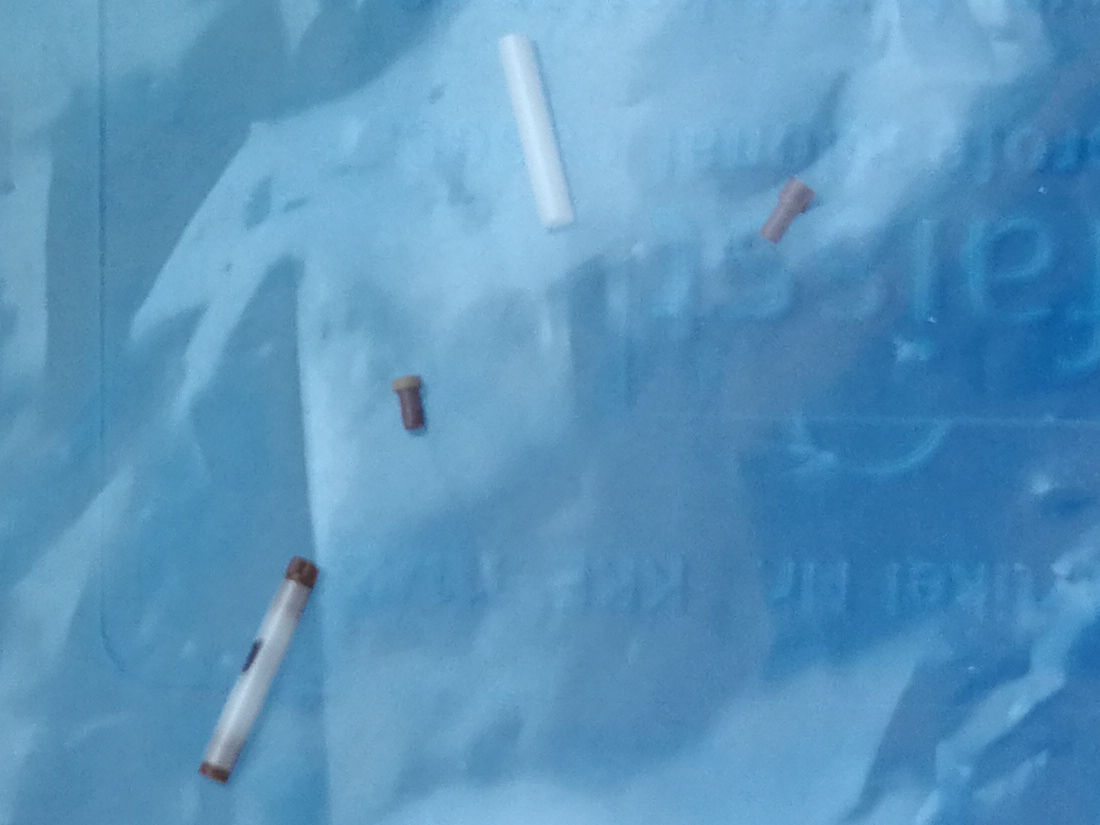
\includegraphics[width=8cm]{images/IMG_20180417_163058_crop.jpg}
					\captionof{figure}{X-ray of patient’s knee, AP an ML view.}
					\label{fig:xray}
				\end{Figure}
			
			\subsection{Resultate}
				\lipsum[1]
			
				\begin{Figure}
					\centering
					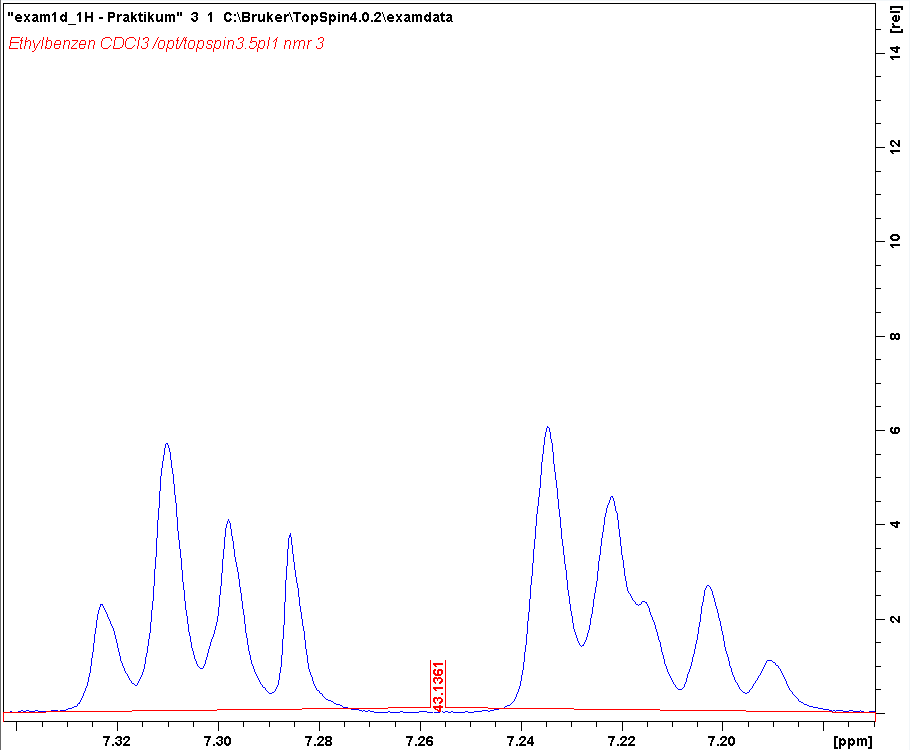
\includegraphics[width=7cm]{images/i_crop.PNG}
					\captionof{figure}{2D reconstruction of some pictures from the CT scan.}
					\label{fig:ct}
				\end{Figure}
				
				\begin{Figure}
					\centering
					\begin{tikzpicture}
						\node[anchor=south west,inner sep=0] at (0,0) {
							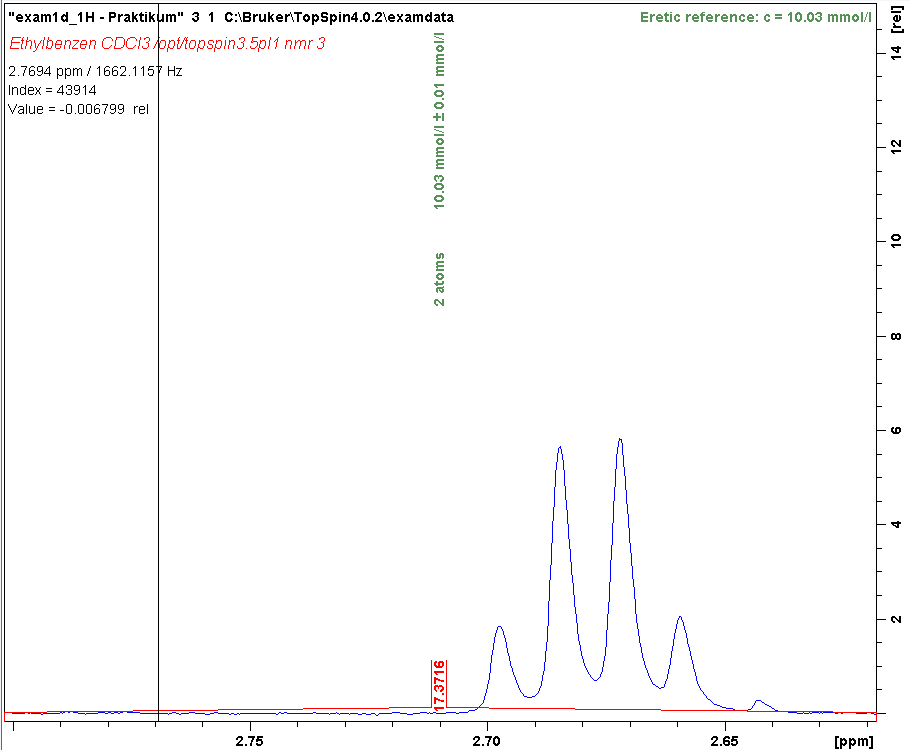
\includegraphics[width=7cm]{images/ii_crop.PNG}
						};
						\draw[red,ultra thick,rounded corners] (0,0) rectangle (1cm,1cm);
					\end{tikzpicture}
					\captionof{figure}{3D reconstruction of some pictures from the CT scan.}
					\label{fig:3d}
				\end{Figure}
				
	
			
	\end{multicols*}
\end{document}